%%%%%%%%%%%%%%%%%%%%%%%%%%%%%%%%%%%%%%%%%%%%%%%%%%%%%%%%%%%%%%%%%%%%%%%%%%%%%%%%%%%%
% Document data
%%%%%%%%%%%%%%%%%%%%%%%%%%%%%%%%%%%%%%%%%%%%%%%%%%%%%%%%%%%%%%%%%%%%%%%%%%%%%%%%%%%%
\documentclass[12pt]{article} %report allows for chapters
%%%%%%%%%%%%%%%%%%%%%%%%%%%%%%%%%%%%%%%%%%%%%%%%%%%%%%%%%%%%%%%%%%%%%%%%%%%%%%%%%%%%
\usepackage{preamble}

\begin{document}

\begin{center}
   \textsc{\large MATH 271, Worksheet 7, \emph{Solutions}}\\
   \textsc{Vectors, vector spaces, and linear transformations.}
\end{center}
\vspace{.5cm}

\begin{problem}
Compare and contrast the structure of the complex numbers $\C$ with the vector space $\R^2$.  Note any differences and similarities. Can you multiply vectors in $\R^2$?
\end{problem}
\begin{solution}
    The algebraic structure of $\C$ and the vector space $\R^2$ are quite similar.  In particular, it was convenient to think of real axis as the $x$-axis and the imaginary axis as the $y$-axis in the plane. A complex number $z=x+iy$ can then be drawn as an arrow based at 0 with a tip at the point $(x,y)$ in the plane. This is analogous to the point $\vecu = x\xhat +y\yhat$ in $\R^2$. 

    Adding two complex numbers $z_1=x_1 + i y_1$ and $z_2 = x_2 + iy_2$ yields 
    \[
        x_1 + x_2 + i(y_1 + y_2),
    \]
    which is a componentwise addition. This addition is the same as taking $\vecu_1 = x_1 \xhat + y_1 \yhat$ and $\vecu_2 = x_2 \xhat + y_2 \yhat$ and computing
    \[
        \vecu_1 + \vecu_2 = (x_1 + x_2) \xhat + (y_1 + y_2)\yhat.
    \]
    Thus, we can also think of addition in both $\C$ and $\R^2$ as attaching the tail $z_1$ to the tip of $z_2$ much like we can do the same with adding $\vecu_2$ to $\vecu_2$ in a geometrical sense.

    Sadly, there is no (nontrivial to explain) notion of multiplication of vectors in \textbf{ANY} vector space.  The closest we achieve is in $\R^3$ with a cross product (though you should not think of this as vector multiplication).  But, we can multiply $z_1 z_2 = x_1 x_2 - y_1 y_2 + i(x_1 y_2 + x_2 y_1)$.  It turns out that we can represent this multiplication (somehow) in $\R^2$, but it requires us to use matrices or something called \emph{geometric algebra}.  I'm a huge proponent of geometric algebra, but it is not a common method of instruction (yet!).
\end{solution}

\newpage
\begin{problem}
Let $\vecu,\vecv\in \R^2$ be given by
\[
\vecu = 2\xhat + 3 \yhat \qquad \textrm{and} \qquad \vecv = -\xhat +\yhat.
\]
\begin{enumerate}[(a)]
    \item Draw $\vecu$, $\vecv$, and $\vecu + \vecv$ in the plane.
    \item Compute $\|\vecu\|$ and $\|\vecv\|$.
    \item Compute $\vecu \cdot \vecv$.
    \item Find a vector orthogonal to $\vecu$.
\end{enumerate}
\end{problem}
\begin{solution}~
    \begin{enumerate}[(a)]
        \item We have the following:
        \[
        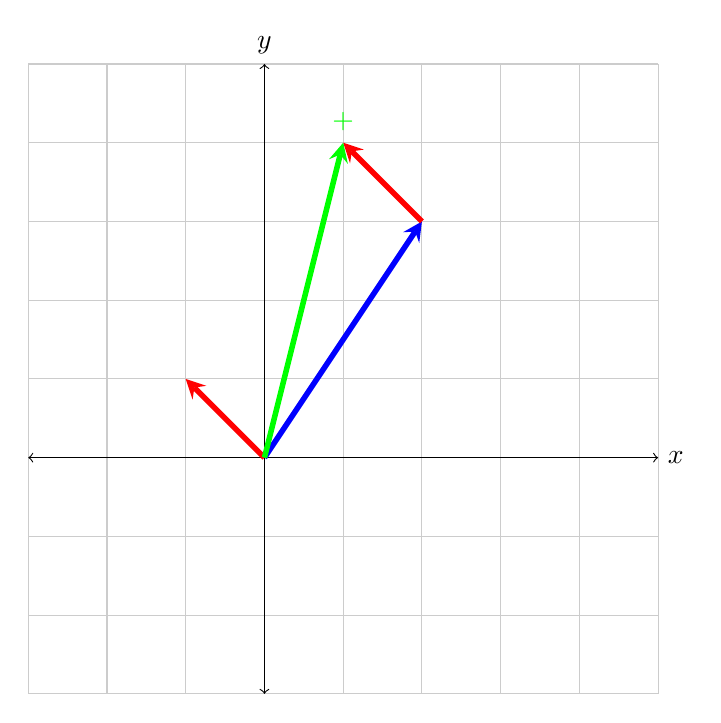
\begin{tikzpicture}
        \draw[thin,gray!40] (-3,-3) grid (5,5);
        \draw[<->] (-3,0)--(5,0) node[right]{$x$};
        \draw[<->] (0,-3)--(0,5) node[above]{$y$};
        \draw[line width=2pt,blue,-stealth](0,0)--(2,3) node[anchor=west] at (2,3){$\vecu$};
        \draw[line width=2pt, red, -stealth](0,0)--(-1,1) node[anchor=east] at (-1,1){$\vecv$};
        \draw[line width=2pt, red, -stealth](2,3)--(1,4) node[anchor=north] at (1,4){};
        \draw[line width=2pt, green, -stealth](0,0)--(1,4) node[anchor=south] at (1,4){$\vecu+\vecv$};
        \end{tikzpicture}
        \]

        \item To compute the lengths we can use the dot product (which amounts to using the pythagorean theorem).  We have
        \[
            \|\vecu\| = \sqrt{\vecu \cdot \vecu} = \sqrt{2^2 + 3^2} = \sqrt{13}
        \]
        and
        \[
            \|\vecv\| = \sqrt{\vecv \cdot \vecv} = \sqrt{(-1)^2 + 1^2} = \sqrt{2}.
        \]

        \item We have
        \[
            \vecu \cdot \vecv = 2(-1)+3(1) = 1.
        \]
        
        \item Consider some vector $\vecw = w_1 \xhat + w_2 \yhat$.  Then, we want $\vecw$ to bo orthogonal to $\vecu$ which means
        \[
            \vecu \cdot \vecw = 0.
        \]
        Hence, we arrive at an (underdetermined) equation
        \[
            0 = 2w_1+3w_2.
        \]
        Clearly, we can take $w_1=0$ and $w_2=0$ to get a trivial answer.  One should note that this yields the $\zerovec$ and $\zerovec$ is always orthogonal to every vector!  To get a nontrivial answer, we note
        \[
            2w_1 = -3w_2 ~\implies~ \frac{w_1}{w_2} = \frac{-3}{2},
        \]
        so finding an orthogonal vector $\vecw$ to $\vecu$ in the plane amounts to just determining the angle that the vector $\vecw$ must have.  We can plot a line in the plane with slope $\frac{-3}{2}$ and see that any vector that lies on this line is orthogonal to $\vecu$.
        \[
        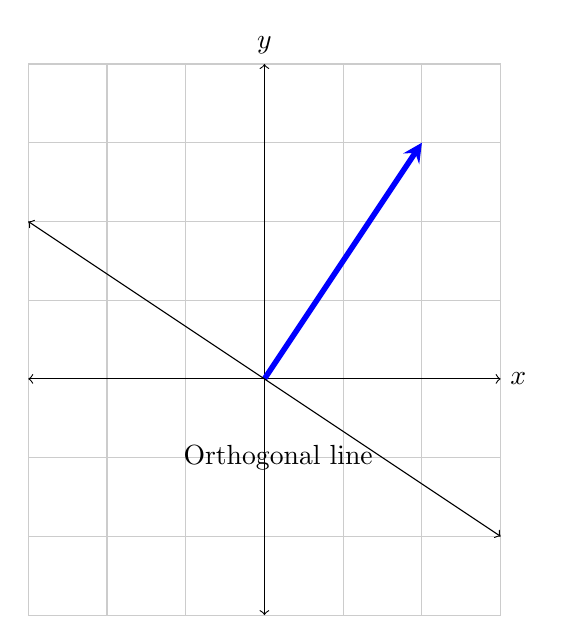
\begin{tikzpicture}
        \draw[thin,gray!40] (-3,-3) grid (3,4);
        \draw[<->] (-3,0)--(3,0) node[right]{$x$};
        \draw[<->] (0,-3)--(0,4) node[above]{$y$};
        \draw[line width=2pt,blue,-stealth](0,0)--(2,3) node[anchor=west] at (2,3){$\vecu$};
        \draw[<->] (-3,2)--(3,-2) node[left] at (1.5,-1){Orthogonal line};
        \end{tikzpicture}
        \]
        So it us up to us to simply choose some vector on this line.  Perhaps the most obvious choice from looking at our equation above yeilds $w_1=-3$ and $w_2=2$ which amounts to the orange vector $\vecw$ shown below.
        \[
        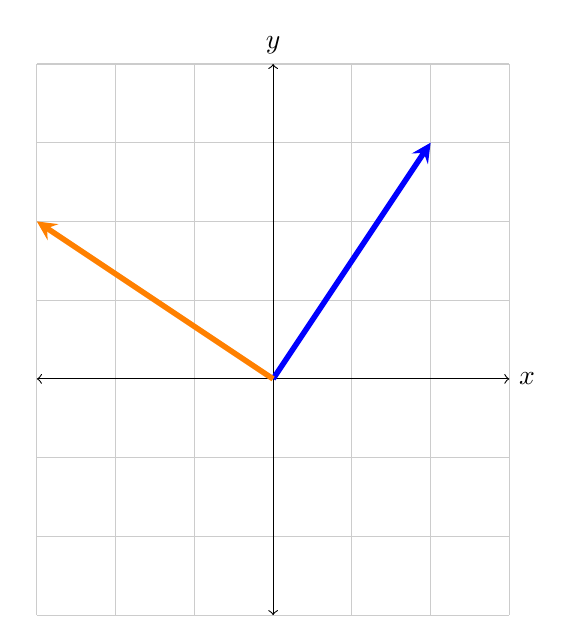
\begin{tikzpicture}
        \draw[thin,gray!40] (-3,-3) grid (3,4);
        \draw[<->] (-3,0)--(3,0) node[right]{$x$};
        \draw[<->] (0,-3)--(0,4) node[above]{$y$};
        \draw[line width=2pt,blue,-stealth](0,0)--(2,3) node[anchor=west] at (2,3){$\vecu$};
        \draw[line width=2pt,orange,-stealth](0,0)--(-3,2) node[anchor=south] at (-3,2){$\vecw$};
        \end{tikzpicture}
        \]
    \end{enumerate} 
\end{solution}

\newpage
\begin{problem}
Let $\vecu,\vecv\in \R^3$ be given by
\[
\vecu = \xhat - \yhat + \zhat \qquad \textrm{and} \qquad \vecv = -\xhat + \yhat - \zhat.
\]
\begin{enumerate}[(a)]
    \item Are $\vecu$ and $\vecv$ orthogonal?
    \item Normalize $\vecu$ and $\vecv$ to get $\uhat$ and $\vhat$. 
    \item Compute the projection of $\vecv$ onto the direction defined by $\vecu$.
\end{enumerate}
\end{problem}
\begin{solution}~
    \begin{enumerate}[(a)]
        \item We can check this by taking the dot product
        \[
            \vecu \cdot \vecv = -1-1-1 = -3,
        \]
        so, no, the vectors are not orthogonal.
        \item To normalize $\vecu$ and $\vecv$ we first compute $\|\vecu\|$ and $\|\vecv\|$.  We have
        \[
            \|\vecu\| = \sqrt{\vecu \cdot \vecu} = \sqrt{1^2+(-1)^2+1^2}=\sqrt{3}
        \]
        and
        \[
            \|\vecv\| = \sqrt{\vecv \cdot \vecv} = \sqrt{(-1)^2+1^2 + (-1)^2} = \sqrt{3}.
        \]
        Then
        \[
            \uhat = \frac{1}{\|\vecu\|} \vecu = \frac{1}{\sqrt{3}} \xhat - \frac{1}{\sqrt{3}} \yhat + \frac{1}{\sqrt{3}} \zhat
        \]
        and
        \[
            \vhat = \frac{1}{\|\vecv\|} \vecv = -\frac{1}{\sqrt{3}} \xhat + \frac{1}{\sqrt{3}} \yhat - \frac{1}{\sqrt{3}} \zhat.
        \]
        \item We can compute the projection of $\vecv$ in the direction of $\vecu$ by computing
        \[
            \vecv \cdot \uhat = \frac{1}{\|\vecu\|} \vecv \cdot \vecu = \frac{-3}{\sqrt{3}}.
        \]
    \end{enumerate}
\end{solution}

\newpage
\begin{problem}
Let $\vecu,\vecv \in \R^3$ be given by
\[
\vecu = -3\xhat -2\yhat + \zhat \qquad \textrm{and} \qquad \vecv = \xhat -2\yhat +\zhat.
\]
\begin{enumerate}[(a)]
    \item Compute the angle between $\vecu$ and $\vecv$.
    \item Without computing the cross product, compute the area of the parallelogram generated by $\vecu$ and $\vecv$. \emph{Hint: you know the angle between the vectors, use this fact.}
    \item Without computing the cross product, what component of the product $\vecu\times\xhat$ must be zero? 
    \item Compute $\vecu\times \vecv$.
    \item Give a geometrical interpretation of the cross product $\vecu\times \vecv$. Explain why $\vecu\times \vecv = -\vecv \times \vecu$.
\end{enumerate}
\end{problem}
\begin{solution}~
    \begin{enumerate}[(a)]
        \item To compute the angle $\theta$ between $\vecu$ and $\vecv$ we need to compute their lengths as well as the dot product between them since $\vecu \cdot \vecv = \|\vecu\|\|\vecv\| \cos \theta$.  So, we get
        \[
            \|\vecu\| = \sqrt{14},\quad \|\vecv\| = \sqrt{6}, \quad \vecu\cdot \vecv = 2.
        \]
        Hence,
        \[
        2 = \sqrt{14}\sqrt{6} \cos \theta
        \]
        and thus
        \[
            \theta = \arccos \left(\frac{2}{\sqrt{14}\sqrt{6}} \right) \approx 1.351 ~\textrm{radians}.
        \]
    \end{enumerate}
\end{solution}

\newpage
\begin{problem}
Recall that the states found in the solution to the free particle in a 1-dimensional box of length $L$ were $\psi_n = \sqrt{\frac{2}{L}} \sin \left( \frac{n\pi x}{L}\right)$. Let $S$ denote the set of all solutions to the free particle in a 1-dimensional box boundary value problem. Show that a superposition of states (with coefficients in $\C$) is \textbf{NOT} a solution. That is, if we let $\Psi(x) = \alpha_{j}(x) \psi_j + \alpha_k \psi_k(x)$, then $\Psi(x)$ is \textbf{NOT} solution to the boundary value problem
\[
-\frac{\hbar^2}{2m}\frac{d^2 \Psi}{dx^2}=E\Psi
\]
with boundary values $\Psi(0)=0$ and $\Psi(L)=0$.
\end{problem}
\begin{solution}
    To see that a superposition of states $\Psi = \alpha_j \psi_j + \alpha_k \psi_k$ is not a solution we must see that $\Psi$ must not satisfy the ODE since $\Psi$ does satisfy the boundary conditions.  In particular,
        \begin{align*}
            -\frac{\hbar^2}{2m} \frac{d^2 \Psi}{dx^2} &=  -\frac{\hbar^2}{2m} \left(\alpha_j \frac{d^2 \psi_j}{dx^2} + \alpha_k \frac{d^2 \psi_k}{dx^2} \right)\\
            &= \alpha_j E_j \psi_j + \alpha_k E_k \psi_k.
        \end{align*}
        So, $\Psi$ does not solve the (time independent) Sch\"odinger equation! Only the states do!  That is why we refer to these as \emph{stationary states}.  One must add time dependence in order for a superposition to be a solution!
\end{solution}

\newpage
\begin{problem}
Consider the transformation $T\colon \R^2 \to \R^3$ given by
\[
T \begin{pmatrix} x \\ y \end{pmatrix} = \begin{pmatrix} x \\ y \\ x+y \end{pmatrix}.
\]
\begin{enumerate}[(a)]
    \item Show that this transformation is linear.
    \item Write down a matrix for this linear transformation.
    \item Can you draw a picture of the output of this transformation? What kind of object is it?
\end{enumerate}
\end{problem}
\begin{solution}~
    \begin{enumerate}[(a)]
        \item To see that this transformation is linear, we consider two vectors $\vecu = \begin{pmatrix} u_1 \\ u_2 \end{pmatrix}$ and $\vecv = \begin{pmatrix} v_1 \\ v_2 \end{pmatrix}$ and a scalar $\alpha \in \R$.  There are two key parts to showing the transformation is linear.
        \begin{itemize}
            \item We show $T(\vecu + \vecv) = T(\vecu) + T(\vecv)$.
            \begin{align*}
                T(\vecu + \vecv) &= T\begin{pmatrix} u_1 + v_1 \\ u_2 + v_2 \end{pmatrix}\\
                &= \begin{pmatrix} u_1 + v_1 \\ u_2 + v_2 \\ u_1 + v_1 + u_2 + v_2 \end{pmatrix}\\
                &= \begin{pmatrix} u_1 \\ u_2 \\ u_1 + u_3 \end{pmatrix} + \begin{pmatrix} v_1 \\ v_2 \\ v_1 + v_2 \end{pmatrix}\\
                &= T(\vecu) + T(\vecv).
            \end{align*}
            So $T$ satisfies the first requirement.
            
        \item Next we show $T(\alpha \vecu)=\alpha T(\vecu)$.
        \begin{align*}
            T(\alpha \vecu) &= T \begin{pmatrix} \alpha u_1 \\ \alpha u_2 \end{pmatrix}\\
            &= \begin{pmatrix} \alpha u_1 \\ \alpha u_2 \\ \alpha u_1 + \alpha u_2 \end{pmatrix} \\
            &= \begin{pmatrix} \alpha u_1 \\ \alpha u_2 \\ \alpha (u_1 +  u_2) \end{pmatrix}\\
            &= \alpha T(\vecu).
        \end{align*}
        So $T$ satisfies the second requirement and thus $T$ is linear.
        \end{itemize}
        \item To find the matrix for $T$, we see how $T$ acts on the vectors $\xhat$ and $\yhat$. We have
        \[
            T(\xhat) = \begin{pmatrix} 1 \\ 0 \\ 1 \end{pmatrix} \qquad \textrm{and} \qquad T(\yhat) = \begin{pmatrix} 0 \\ 1 \\ 1 \end{pmatrix}.
        \]
        Thus, the columns for the matrix $[T]$ are given by $T(\xhat)$ and $T(\yhat)$.  Specifically,
        \[
            [T] = \begin{pmatrix} \vert & \vert \\ T(\xhat) & T(\yhat) \\ \vert & \vert \end{pmatrix} = \begin{pmatrix} 1 & 0 \\ 0 & 1 \\ 1 & 1 \end{pmatrix}.
        \]
        \item The picture could look something like this.
        \begin{center}
\tdplotsetmaincoords{60}{120} 
\begin{tikzpicture} [scale=3, tdplot_main_coords, axis/.style={->,black,thick}, 
vector/.style={-stealth,blue,very thick}, 
vector guide/.style={dashed,red,thick}]

%standard tikz coordinate definition using x, y, z coords
\coordinate (O) at (0,0,0);

%tikz-3dplot coordinate definition using x, y, z coords

\pgfmathsetmacro{\ax}{0.6}
\pgfmathsetmacro{\ay}{1}
\pgfmathsetmacro{\az}{0.8}

\coordinate (P) at (\ax,\ay,\az);

%draw axes
\draw[axis] (0,0,0) -- (2,0,0) node[anchor=north east]{$x$};
\draw[axis] (0,0,0) -- (0,2,0) node[anchor=north west]{$y$};
\draw[axis] (0,0,0) -- (0,0,2) node[anchor=south]{$z$};


\draw[line width=2pt, red, -stealth](0,0,0)--(0,1,0) node[anchor=north west] at (0,1,0){$\yhat$};
\draw[line width=2pt, blue, -stealth](0,0,0)--(1,0,0) node[anchor=north] at (1,0,0){$\xhat$};
\draw[line width=2pt, purple, -stealth](0,0,0)--(1,0,1) node[anchor=east] at (1,0,1){$T(\xhat)$};
\draw[line width=2pt, orange, -stealth](0,0,0)--(0,1,1) node[anchor=west] at (0,1,1){$T(\yhat)$};

\end{tikzpicture}
\end{center}
\begin{center}
\tdplotsetmaincoords{60}{120} 
\begin{tikzpicture} [scale=3, tdplot_main_coords, axis/.style={->,black,thick}, 
vector/.style={-stealth,blue,very thick}, 
vector guide/.style={dashed,red,thick}]

\end{tikzpicture}
\end{center}
        The output of this transformation is a vector in $\R^3$.  So we are taking planar vectors and converting them to new vectors that live in space.
    \end{enumerate}
\end{solution}



\end{document}
